\chapter{Sequence Prediction with Traces}
\label{chap:taking-inspiration}
Previous works have demonstrated the practicality of LSTM neural networks for predictive process monitoring. However, only the use of embedding layers was inspired by natural language processing (NLP) until now~\cite{evermann2016}. We believe that more knowledge could be transferred because both domains revolve around sequential data. In this chapter, we outline how we take inspiration from sequence prediction in NLP, and thus contribute to Improvement Area 1 (NLP-influence) from \autoref{sec:intro:motivation}.

We establish the connection between traces and sequences by connecting their definitions in \autoref{sec:contrib:case-sequence-understanding}. This provides the underpinning for introducing two NLP-inspired approaches for predicting the next activity in a case. These approaches are presented in \autoref{sec:contrib:sp2-inspiration} and \autoref{sec:contrib:pfs-inspiration}.

\section{Understanding Traces as Sequences}\label{sec:contrib:case-sequence-understanding}
The definition for sequences presented in \autoref{sec:background:sequences} and the definition of traces in \autoref{sec:log-structure} will be connected in this section to make it clear how events can be understood as itemsets.

Events are ordered in traces, and each case $c$ contains its execution history in its trace attribute $\#_{trace}(c)$.
Similarly, a sequence $seq$ is defined to contain itemsets in an ordered fashion:

\begin{equation*}
\begin{split}
seq           &=  \langle s_1,s_2\cdots s_l \rangle\ |\ \forall\ 1 \leq j \leq l: s_j \subseteq \mathscr{I}\\
\#_{trace}(c) &= \langle e_1, e_2, e_3\cdots e_n \rangle
\end{split}
\end{equation*}

An itemset $s = (i_1, i_2 \cdots i_n)$ consists of items $i \in \mathscr{I}$, and is defined as $s \subseteq \mathscr{I}$.
An event $e$ is made up of attributes that are accessed via the $\#$ operator.
It can be said that both itemsets and events act as containers of information.
Therefore, we connect the definitions of the contained information in a first step.
The set of items $\mathscr{I}$ is then defined as the set of all attributes of all events in all cases in a given log $L$:

$$\mathscr{I} = \{\#_{a}(e)\ |\ c \in L\wedge e \in \#_{trace}(c) \wedge a \in attribute\_names(e)\}$$

The definition of itemsets $s \subseteq \mathscr{I}$ does not place any restrictions on the content of $s$,
so an itemset could consist only out of timestamps.
To prevent such cases, we introduce a schema on the itemsets in a second step.
It is introduced as a direct mapping from an event $e$ to an itemset $s$:

$$ s = (i_1, i_2 \cdots i_n)\ |\ i_k = \#_{attribute\_names_k(e)}(e), 1 \leq k \leq n $$

The definition places each item $i_k$ on a specific place in the itemset, depending on the index $k$ in the attribute list $attribute\_names(e)_k$.
The original condition $s \subseteq \mathscr{I}$ hold true.
This definition enables sequence prediction on traces, and also provides the tabular format required for machine learning.

In \autoref{sec:background:sequence-prediction}, a many-to-one prediction is defined to target the next itemset $\widehat{s_{k+1}}$ of any sequence $seq_{1,k}$.
In the use case at hand, this would entail the prediction of all data attributes in $\widehat{s_{k+1}}$.
Since we specifically target the name of the next activity, we adjust the definition of the prediction function to target a single item $\hat{i_j}$.
The index $j$ corresponds to the column index of the target variable inside the itemset $s_{k+1}$, i.e., the index of the activity name in our case.

$$ predict(seq_{1,k}) = \hat{i_j} $$

With the prediction target at hand, we move on to present the network architectures for executing the prediction.

\section{Adapting a Competition Submission}\label{sec:contrib:sp2-inspiration}
Shibata et al.'s bipartite network architecture has shown outstanding performance in the Sequence Prediction challenge (SPiCe)~\cite{web:spice}.
In the last section we have shown that a case trace can also be understood as a sequence, and thus we adapt Shibata's approach for use in the business process domain.

\begin{figure}[!htb]
    \centering
    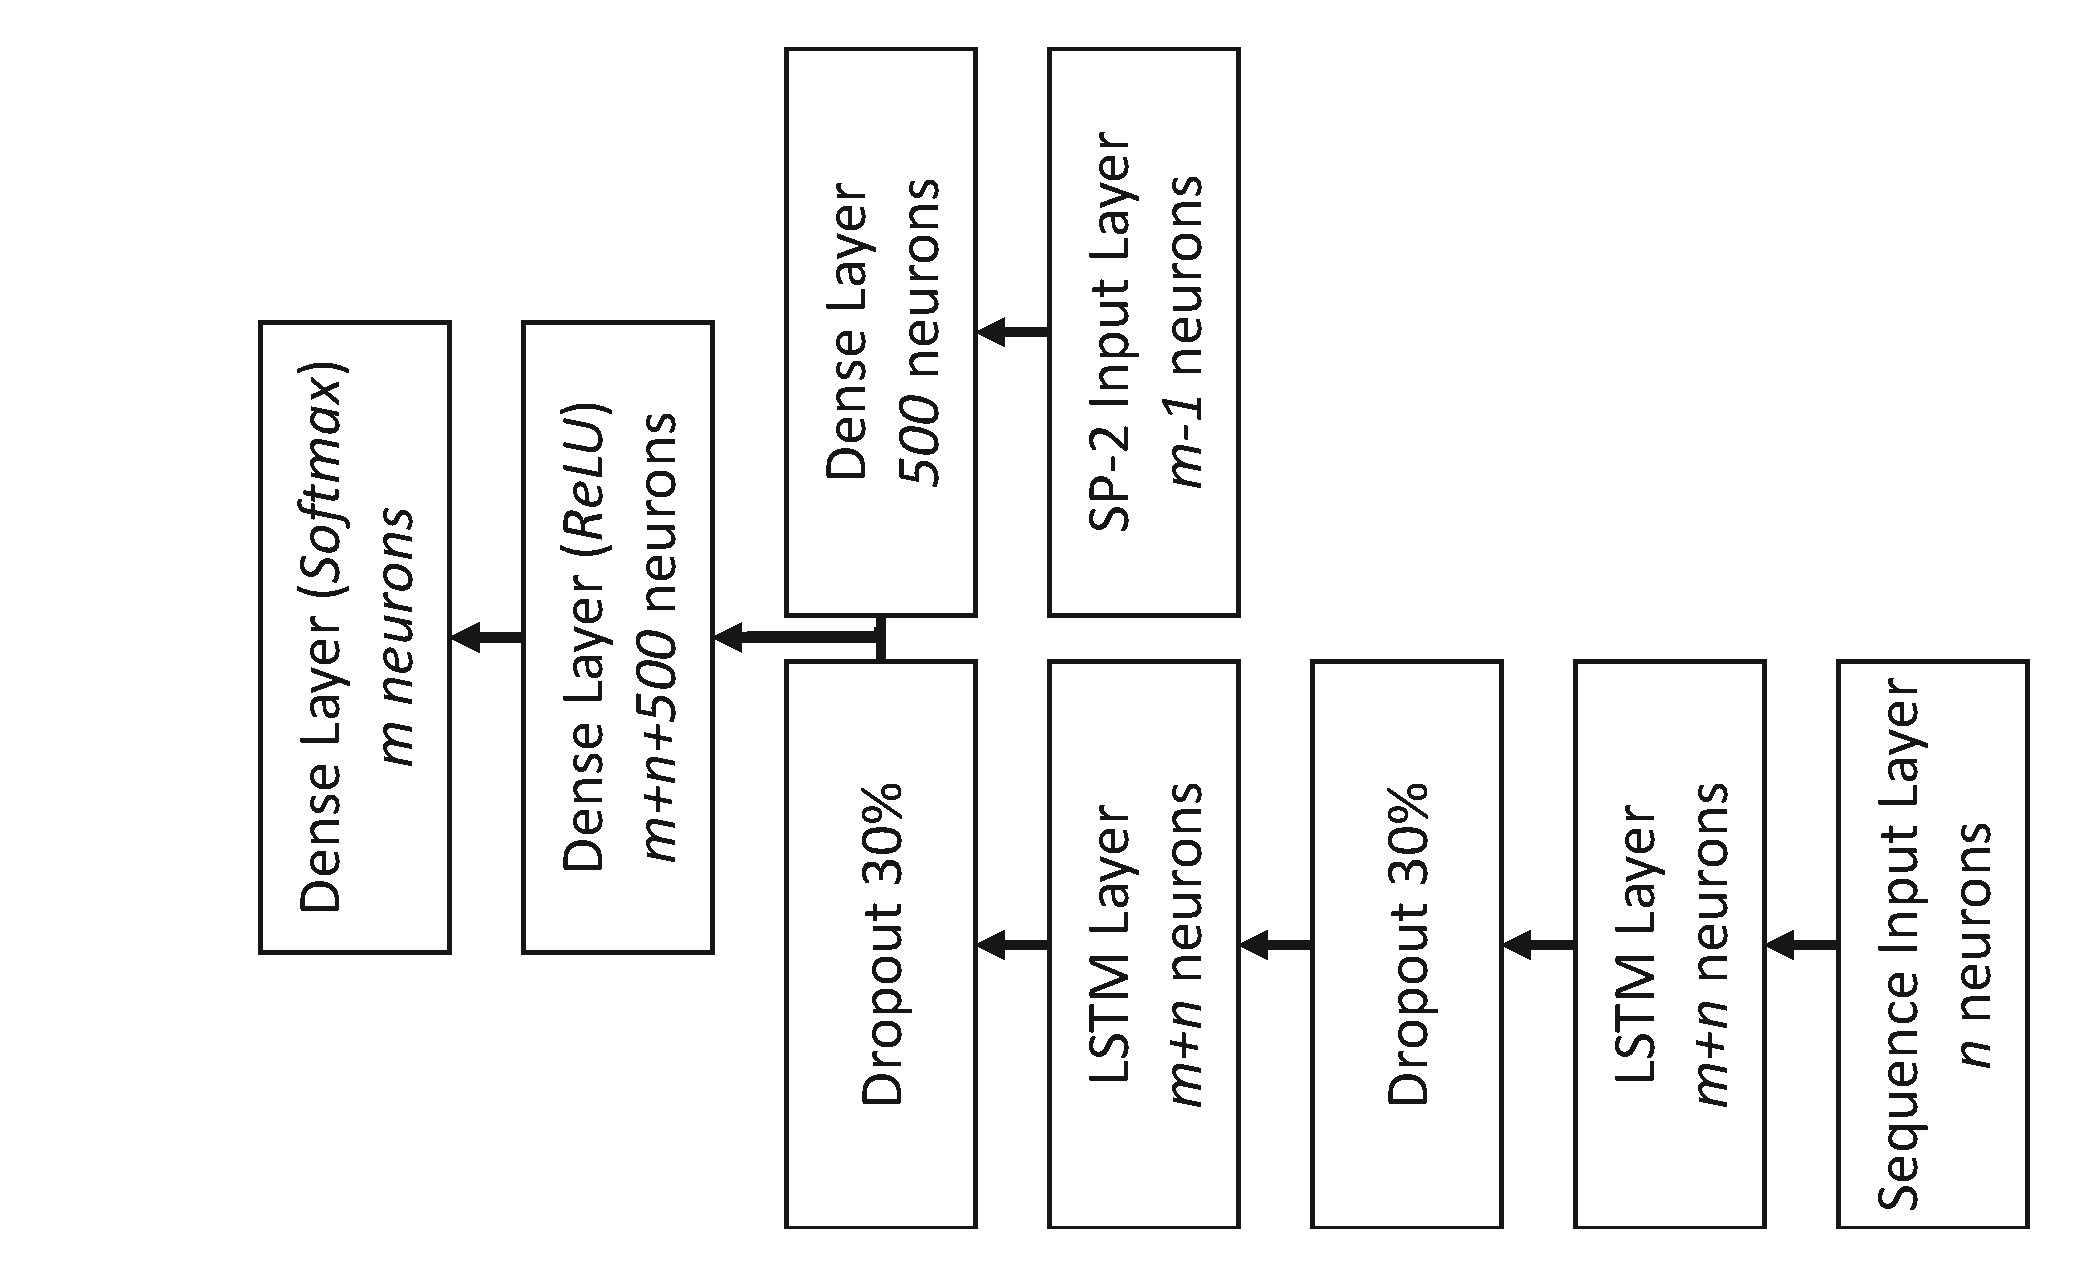
\includegraphics[width=.8\textwidth, angle=-90,origin=c]{gfx/sp2-network-architecture.pdf}
    \caption{The SP2 network architecture}
    \label{fig:sp2-architecture}
\end{figure}

\autoref{fig:sp2-architecture} displays the adapted network architecture from Shibata et al. It is referred to as SP2 from here on.

We copied the bipartite structure and made small changes to dimensions and layers.
The sequential feature vectors, i.e., all event attributes, are fed into the left input layer.
$n$ indicates the dimensionality of the event feature vector, which contains the encoded activity name, timestamp and other data attributes of the respective step.
The sequential data passes through two LSTM layers interleaved with dropout layers to prevent overfitting.
Hidden layers contain $n+m$ neurons, making their size dependent on the input and output dimensions.
This cue was taken from Schönig et al.~\cite{schoenig2018}.
The LSTM layer output is concatenated with the output of the processed SP-2 features for each timestep, which were fed in on the right side of the tree and preprocessed by a feedforward layer.
The concatenated vectors are passed through a ReLU-activated feedforward layer, and finally to the output layer.
A Softmax activation function is applied to the output layer, putting out the next activity in one-hot encoded form through $m$ neurons.
This models the problem as a multi-classification problem.

In contrast to the original model, we completely removed the embedding layers.
Above the SP-2 feature input layer, the embedding layer was replaced with a feedforward layer.
We argue that embedding layers are not necessary for this context, because the number of activity names in a process is small compared to the number of words usually processed with embedding layers in NLP scenarios.


Another difference is the dimensionality $n+m$ of the hidden layers.
In contrast to Evermann et al. and Shibata et al., we do not fix it or make it smaller than the output unit count $m$.
This follows general advice not to introduce bottlenecks in the hidden layers by using fewer units than required in the output layer~\cite{web:techniques-in-convnets,szegedy2016rethinking}.\\

\noindent Shibata et al. engineered their SP-2 features from prediction targets~\cite{shibata2016bipartite}.
Therefore, we produce the SP-2 features from the sequence of activity names.
An exemplary SP-2 feature vector from activity names is depicted in \autoref{tab:sp2-activity-trace}.
It is based on a trace from a case $c$, which contains numeric activity names.


\begin{table}[!htb]
    \centering
    \begin{adjustbox}{center}
    \begin{tabular}{cclccccccccc}
          &      &              & \multicolumn{9}{c}{SP-2 vector}\\
 t & $seq_{t, t}$ & $seq_{0,t}$ & [1 & 2 & 3 & 4 & 5 & 6 & 7 & 8 & 9]\\
        \midrule
        0 & 1    & 1            & [1 & 0 & 0 & 0 & 0 & 0 & 0 & 0 & 0]\\
        1 & 8    & 18           & [1 & 0 & 0 & 0 & 0 & 0 & 0 & 1 & 0]\\
        2 & 6    & 186          & [1 & 0 & 0 & 0 & 0 & 1 & 0 & 1 & 0]\\
        3 & 8    & 1868         & [1 & 0 & 0 & 0 & 0 & 1 & 0 & 1 & 0]\\
        4 & 6    & 18686        & [1 & 0 & 0 & 0 & 0 & 1 & 0 & 1 & 0]\\
    \end{tabular}
    \end{adjustbox}
    \caption[SP-2 features created from an activity trace]{SP-2 features created from an activity trace $seq=\#_{trace}(c)=\langle (1), (8), (6), (8), (6)\rangle$}
    \label{tab:sp2-activity-trace}
\end{table}


\section{Encoding Subsequence Occurrence}\label{sec:contrib:pfs-inspiration}
Klinkmüller et al. compared different feature representations and found that features that encode sub-trace occurrence can help models cover a broader variety of relationships~\cite{klinkmuller2018reliablemonitoring}.
While they found this to be true for random forests, we want to investigate the applicability of such features with LSTM neural networks.
Francescomarino et al. tried this in their work and achieved discouraging accuracies around $0.50$~\cite{francescomarino2017}.
We are convinced that another network architecture could make a difference.

SP-2 features already encode history and subsequence encodings do the same on a higher level of abstraction.
Therefore, we take the SP2 model architecture and inject different features in place of the SP-2 features.
The respective architecture is shown in \autoref{fig:pfs-architecture}.

\begin{figure}
    \centering
    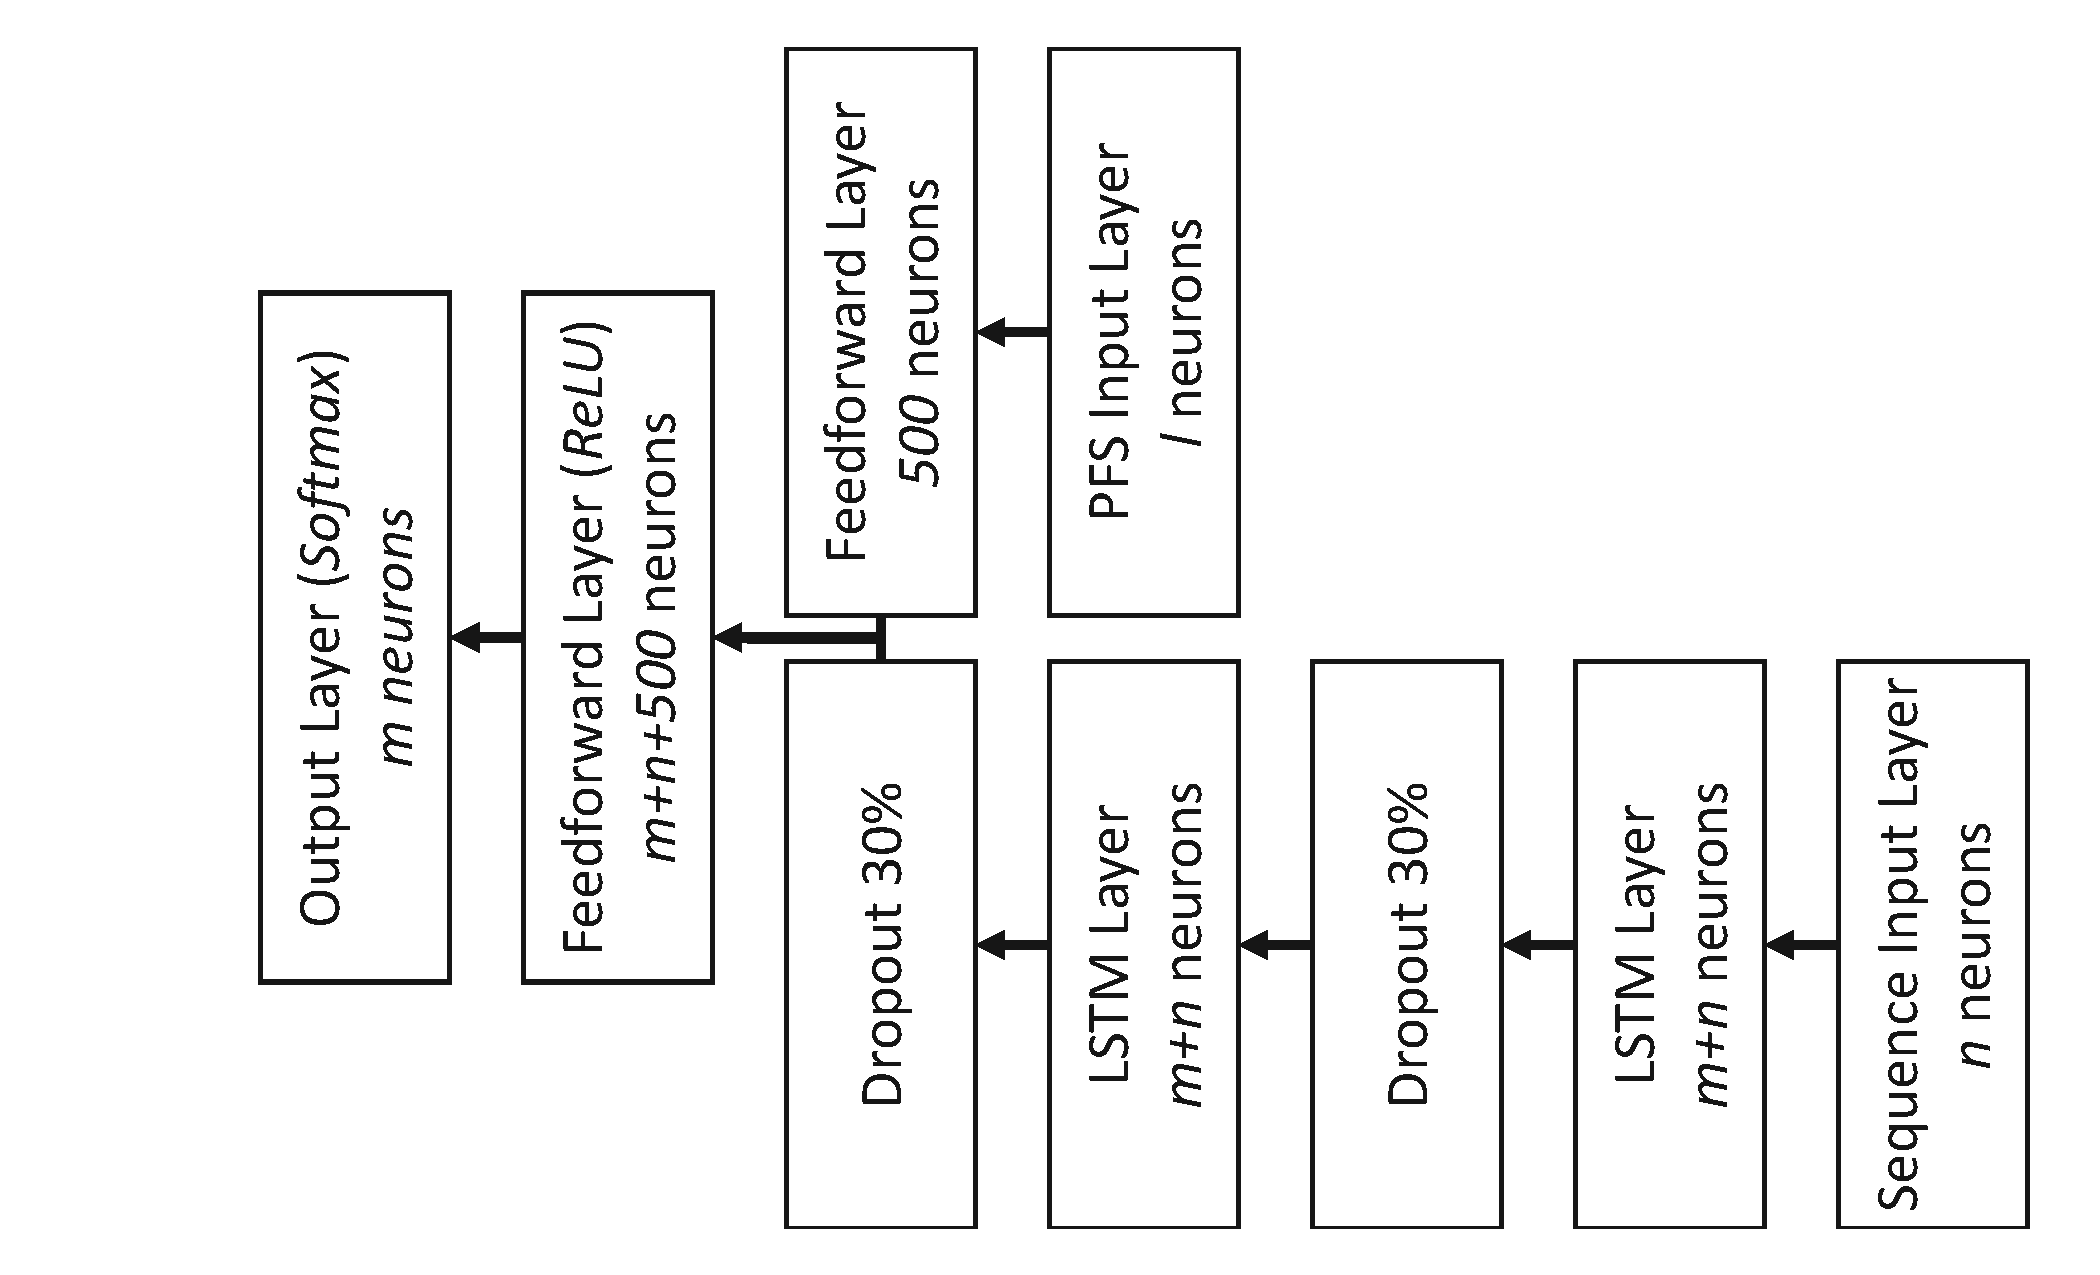
\includegraphics[width=.8\textwidth,angle=-90,origin=c]{gfx/pfs-network-architecture.pdf}
    \caption{The PFS network architecture}
    \label{fig:pfs-architecture}
\end{figure}

We will henceforth refer to both the architecture and the subsequence features as PFS.
The acronym PFS originates from the word PrefixSpan, which is the name of the algorithm that we use later to mine the subsequences.
The PFS feature vector has $l$ dimensions and is fed in on the right side of the tree.

The PFS vector encodes whether common subsequences have occurred yet, as \autoref{tab:pfs-activity-trace} illustrates.
The illustration is based on the trace $seq=\#_{trace}(c)=\langle (1), (8), (6), (8), (6)\rangle$.
From the log that $seq$ was taken from, we mined four common subsequences: $\langle 6\rangle$, $\langle 1,6\rangle$, $\langle 8,6\rangle$, and $\langle1,8,6\rangle$.
In the example, a field inside the feature vector is set to 1 when the respective subsequence has occurred.\\

We presented two neural network architectures in this chapter. They incorporate
learnings from a successful NLP competition submission, and a paper on feature engineering.
Training these models on a multitude of datasets presented us with a challenge.
We solved it by constructing a small training framework which we present in the next chapter.

\begin{table}
    \centering
    \begin{adjustbox}{center}
    \begin{tabular}{cclcccc}
          &      &              & \multicolumn{3}{c}{PFS vector}\\
 t & $seq_{t, t}$ & $seq_{0,t}$ & [$\langle 6\rangle$ & $\langle 1,6\rangle$ & $\langle 8,6\rangle$ & $\langle1,8,6\rangle$]\\
        \midrule
        0 & 1    & 1            & [0 & 0 & 0 & 0]\\
        1 & 8    & 18           & [1 & 0 & 0 & 0]\\
        2 & 6    & 186          & [1 & 0 & 1 & 1]\\
        3 & 8    & 1868         & [1 & 0 & 1 & 1]\\
        4 & 6    & 18686        & [1 & 0 & 1 & 1]\\
    \end{tabular}
    \end{adjustbox}
    \caption{PFS features created from an activity trace}
    \label{tab:pfs-activity-trace}
\end{table}
